
\documentclass[letterpaper,twocolumn,10pt]{article}
\usepackage{usenix2019_v3}

% to be able to draw some self-contained figs
\usepackage{tikz}
\usepackage{amsmath}
\usepackage{pgfplots}
\def\code#1{\texttt{#1}}
% inlined bib file
\usepackage{filecontents}

\begin{document}
%-------------------------------------------------------------------------------

%don't want date printed
\date{}

% make title bold and 14 pt font (Latex default is non-bold, 16 pt)
\title{\Large \bf General Matrix Multiplication (GEMM) with the MPI}

%for single author (just remove % characters)
\author{
{\rm Robert Geil}\\
University of California, Los Angeles
} % end author

\maketitle

%-------------------------------------------------------------------------------
\begin{abstract}
%-------------------------------------------------------------------------------
General Matrix Multiplication (GEMM) is an important problem type in many fields
of computer science and is therefore a good candidate for optimization and
parallelization. One approach to parallelization is using the Message Passing
Interface (MPI). This system allows the use of Single Program-Multiple Data
(SPMD), allowing extremely large numbers of processors to be programmed with a
single program. In this lab, we simulated a cluster on a single machine, and via
MPI were able to improve the efficiency of multiplication of matricies reaching
a peak of $\approx 160$ GFlops.
\end{abstract}

%-------------------------------------------------------------------------------
\section{Introduction}
%-------------------------------------------------------------------------------

While local multithreading can give a significant performance
gain in domains such as GEMM, it is limited by the size of shared memory and the
number of cores on a chip. In practice, this means that OpenMP and other
multithreading systems can only support at most dozens of cores. However data
may scale to be many gigabytes, terrabytes or even more. To process such a
large quanitity, we must use another programming paradigm, which is where MPI
comes in. Unlike OpenMP, MPI requires the explicit transmission of data between
machines (or cores in our case), and provides many primitives to perform such
communication as \textbf{scatter} to break up data and send to each worker,
\textbf{broadcast} to replicate data among all threads and \textbf{gather} to
condense data back to a single processor. By using these in conjunction with
more typical optimizations like cache, we can improve the performance of our
test machine, which would translate to an even larger improvement on a
machine like a supercomputer with more physical CPUs.

%-------------------------------------------------------------------------------
\section{Machine Specifications}
%-------------------------------------------------------------------------------

As with lab 1, the machine for which the code was optimized is an Amazon Web 
Services (AWS) \textit{m5.2xlarge} virtual machine. This machine has 4 virtual 
CPUs, each of which supports 2 threads via Intel's Hyperthreading technology. 
The processor is clocked at 3.1 GHz, and contains 32 Kb L1, 1024 Kb L2 and 
33792 Kb L3 cache. In addition, the cache line size was 64 bytes.

%-------------------------------------------------------------------------------
\section{Solution Approach}
%-------------------------------------------------------------------------------
In order to deliver the improvement required, we had to optimize both 
communication between processors as well as the computation on the individual
cores.

\subsection{Unbuffered vs. Buffered vs. Non-Blocking}
MPI provides primitives to communicate either unbuffered, with a buffer, or in
a non-blocking format. There are benefits and drawbacks to each of these, both
in a programming and in a performance perspective. For the standard, unbuffered
communcication, the messages are sent synchronously, which requires a receiver
to be waiting for each sender, otherwise there will be a deadlock. However, it
guarantees that the data has reached the other processor once execution
continues in the sender. With Buffered communication, this can add performance
improvements with some applications where the sender and receiver aren't
totally in sync, and by having a buffer, the sender can proceed to other tasks
without having to wait for the receiver's confirmation. A drawback to this is
that buffer sizes are finite, and therefore may cause an issue if one process
is generating data faster than another can consume it. Finally non-blocking can
send data and allow the sender to immediately carry on with other tasks, but
this introduces issues of synchronization, where the sender may need to perform
some waiting or other explicit instruction, adding to programmer burden.

\subsection{Communication}
For our purposes, the data are split among the processors from array $a$, and
array $b$ is broadcast among all processors. Using this approach, each process
multiplies its portion of $a$ against all of $b$, and then the results can be
gathered back to the root process. We utilized the MPI functions 
\code{MPI\_Scatter} to send $a$, \code{MPI\_Bcast} to send $b$ and 
\code{MPI\_Gather} to return the results to the root process. These were used
to split up $a$, broadcast $b$ and gather back $c$ respectively. The MPI 
functions utilize a multiplicative system to transmit and gather data, giving
only $\log(n)$ sets of communication for $n$ processors. While that doesn't
make a huge impact in our set of only 4 cores, it has a profound impact in
larger data centers, where something like 1 million cores could scatter data
in around 20 steps. In terms of physical communication, since we are simulating
a cluster, our data are transmitted across shared memory using interprocess
communication through the kernel. However, in a larger datacenter, an
interconnect such as Ethernet or infiniband may be used between nodes.

\subsection{Matrix Multiplication}
The actual matrix multiplication was approached with a couple of optimizations.
First, loop ordering and blocking, as done in the previous lab helped to improve
cache hit rates. Secondly, the memory that was traversed over was allocated 
using \code{aligned\_alloc()} rather than a traditional memory allocation
function. This allows the memory to align better with cache lines, letting the
processing of blocks be done within cached data. Finally, we used loop unrolling
and some optimization (eg shifts and adds rather than multiplication) within
the innermost loop, giving us our final optimized performance.

%-------------------------------------------------------------------------------
\section{Results}
%-------------------------------------------------------------------------------
\subsection{Performance}
As can be seen from figure~\ref{fig:size}, this solution benefits from scaling
up of data. With the same number of processors, the $4096^3$ performance is
almost three times as good as that of the $1024^3$ problem. The main reason for
this improvement is the relative proportion of the compute time that must be
spent on communication. Since we are transmitting the entire $b$ array and part
of the $a$ array, the number of elements that must be transmitted is 
$\approx n^2$ where $n$ is the length of one side of the matrix. However, the
number of operations that each processor must do is on the order of 
$\approx n^3/p$ where $p$ is the number of processors. As such, we see that as
$n$ grows, the amount of processing done grows cubically, while the amount of
data to be transmitted grows quadratically. Therefore, in the long run we
expect that as $n$ grows, more time will be spent on computation, improving our
GFlops.
\begin{figure}
  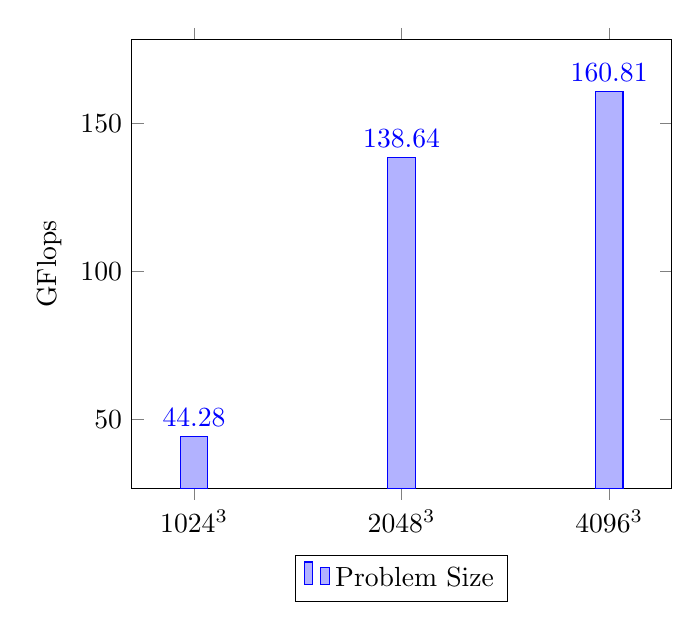
\begin{tikzpicture}
    \begin{axis}[
        ybar,
        enlargelimits=0.15,
        legend style={at={(0.5,-0.15)},
          anchor=north,legend columns=-1},
        ylabel={GFlops},
        symbolic x coords={$1024^3$,$2048^3$,$4096^3$},
        xtick=data,
        nodes near coords,
        nodes near coords align={vertical},
        ]
        \addplot coordinates {($1024^3$,44.28) ($2048^3$,138.64) ($4096^3$,160.81)};
    \legend{Problem Size}
    \end{axis}
    \end{tikzpicture}
    \caption{\label{fig:size} Performance of the MPI GEMM with 4 processors
    on various matrix sizes}
\end{figure}
%-------------------------------------------------------------------------------
\subsection{Scalability}
Figure~\ref{fig:processors} shows that as the number of processors increases,
the throughput increases as well until reaching 4, after which it sharply drops
off. The main reason for this dropoff is that the physical machine only has 4
cores, meaning that any additional processes must be context-switched in. This
introduces overhead and invalidates caches, slowing performance further.
Additionally, we see that below 4 processors, there is a non-linear scaling.
This is due to how the program was set up. Since we send the entire $b$ array
and a strip of the $a$ array, the communication burden grows with the number of
processors, making this solution not very scalable. Another solution which may
be better would be to use tiling of both $a$ and $b$, thereby creating blocks
which may be communicated back. This would then reduce the communication burden
by a factor of the number of processors, helping drive scalability. Indeed, this
was the approach I initially attempted, but having 3 midterms this week ended up
taking a lot of time, forcing me to fall back on this sub-optimal implementation.
\begin{figure}
  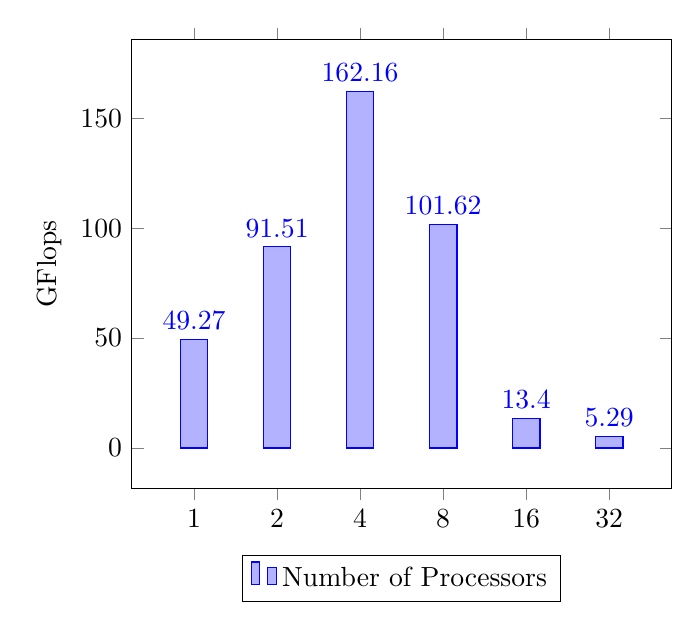
\begin{tikzpicture}
    \begin{axis}[
        ybar,
        enlargelimits=0.15,
        legend style={at={(0.5,-0.15)},
          anchor=north,legend columns=-1},
        ylabel={GFlops},
        symbolic x coords={1,2,4,8,16,32},
        xtick=data,
        nodes near coords,
        nodes near coords align={vertical},
        ]
        \addplot coordinates {(1,49.27) (2,91.51) (4,162.16) (8,101.62) (16,13.40) (32, 5.29)};
    \legend{Number of Processors}
    \end{axis}
    \end{tikzpicture}
    \caption{\label{fig:processors} Performance of the MPI GEMM with 
    different numbers of processors on $4096^3$ matrices}
\end{figure}
%-------------------------------------------------------------------------------
\section{OpenMP Comparison}
OpenMP, as discussed in the introduction, is intended to be used for a single
machine with multiple cores, and therefore has limits to scaling, whereas MPI
can be used for many thousands or millions of independent processors. In terms
of programming effort, OpenMP is by far the easier system to use and integrate
into existing code. Since it uses an incremental approach, and memory is already
shared, by adding a few preprocessor directives, the code can be quickly
parallelized. Since MPI requires explicit sending of messages, more programmer
effort is required, and it is generally harder to approach incrementally. As
for performance, on a large scale MPI will deliver better performance as it can
be used with nearly unlimited resources. For our purposes, MPI was also faster
than OpenMP by roughly 50 GFlops. One potential reason is my use of
\code{aligned\_alloc()} which I was unaware of in the first lab. Another
possibility is that since each processor has its own copy of memory, especially
the $c$ result array, when one processor writes to it, it won't invalidate the
cache of another array, which means the MPI version with segmented memory can
have faster performance via fewer cache misses.
%-------------------------------------------------------------------------------
\end{document}
%%%%%%%%%%%%%%%%%%%%%%%%%%%%%%%%%%%%%%%%%%%%%%%%%%%%%%%%%%%%%%%%%%%%%%%%%%%%%%%%